%! Author = Michał_Komputer
%! Date = 14.10.2021

% Preamble
\documentclass[a4paper,11pt]{article}

% Packages
\usepackage[T1]{fontenc}
\usepackage[backend=bibtex,style=alphabetic]{biblatex}
\usepackage[polish]{babel}
\usepackage[utf8]{inputenc}
\usepackage{amsmath}
\usepackage{array}
\usepackage{enumerate}
\usepackage{float}
\usepackage{graphicx}
\usepackage{indentfirst}
\usepackage{latexsym}
\usepackage{mathtools}
\usepackage{placeins}
\usepackage{polski}
\usepackage{tabularx}


% Title page
\title{Optymalizacja hiperparametrów procesu uczenia sieci neuronowych z wykorzystaniem algorytmu genetycznego}
\author{Michał Zawadzki}
\date{Listopad 2021}


% Additial settings
\DeclareUnicodeCharacter{266D}{
\includegraphics[height=1ex]{music_flat_sign}}
\DeclareUnicodeCharacter{266F}{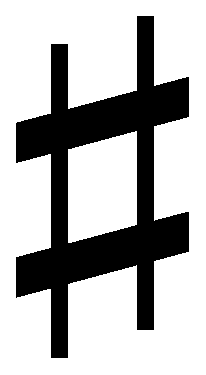
\includegraphics[height=1ex]{music_sharp_sign}}
\addbibresource{references.bib}
\restylefloat{table}

% Document
\begin{document}

    \maketitle

    \tableofcontents


    \section{Wstęp}

    \subsection{Cel pracy}
    Korzystając ze zbioru danych o utworach muzycznych dostępnych na platformie streaming-owej Spotify, stworzono kilka modeli szacujących jaką popularność osiągnie na tej platformie nowy utwór. Modele te są prostymi sieciami neuronowymi o różnej architekturze. Do optymalizacji ich hiperparametrów uczenia wykorzystano algorytm genetyczny.

    \subsection{Teza główna} % uwaga od promotora: jeżeli piszesz tezę to musi być ona znacznie bardziej konkretna, musi opisywać coś mierzalnego
    Algorytm genetyczny może znacząco przyspieszyć proces wyboru optymalnych hiperparametrów uczenia dla wstępnie zaprojektowanej sieci neuronowej.

    \subsection{Słowa kluczowe} % między 5 a 10

    \subsection{Abstrakt} % bardzo skondensowane streszczenie pracy z użyciem słów kluczowych


    \section{Wpływ cech utworów muzycznych na popularność}

    Zaczynając rozważania nad przyczynami, które sprawiają, że niektóre utwory muzyczne osiągają ogromną popularność, podczas gdy inne nie zdobywają uznania szerokiego audytorium, trzeba najpierw zdefiniować podstawowe czynniki jakimi kieruje się odbiorca przy dokonywaniu wyborów muzycznych. Magdalena Parus-Jankowska i Szymon Nożyński w swojej pracy ``Preferencje Muzyczne w Dobie Popularności Strumieniowego Słuchania Muzyki''\cite{PreferencjeMuzyczneWCzasachSteamingu2020} wymieniają 3 takie czynniki:
    \begin{itemize}
        \item \textit{upodobania} - Przywiązanie do konkretnych gatunków muzycznych, wraz z otaczającym je kontekstem kulturowym.
        \item \textit{smak/gust} - Umiejętność dostrzegania i oceny poszczególnych elementów składowych utworu, także znajomość i zrozumienie przesłania utworu.
        \item \textit{preferencje} - Upodobanie dla konkretnych utworów lub twórców muzycznych.
    \end{itemize}

    \smallskip

    Czynniki te często kształtują się równolegle i przenikają znaczeniowo, dlatego też dla uproszczenia w dalszej części posłużono się szeroko rozumianym pojęciem preferencji muzycznych.

    \bigskip

    Preferencje muzyczne człowieka nie są czymś stałym. Zmieniają się one przez całe życie, szczególnie intensywnie w wieku dziecięcym i w okresie dojrzewania\cite{PreferencjeMuzyczneWCzasachSteamingu2020}.Wielki wpływ na sposób konsumpcji treści muzycznych ma środowisko, z którego człowiek się wywodzi, jego wykształcenie, zamożność, światopogląd i osobowość\cite{PreferencjeMuzyczneWCzasachSteamingu2020}. Muzyki słuchają najczęściej ludzie młodzi (w grupie wiekowej 18-24 lata 77\% deklarowało słuchanie muzyki codziennie\cite{cbos2018}) i to oni pośrednio, a bezpośrednio wywodzący się z tej grupy twórcy, kształtują nowe trendy i czynią rynek muzyczny bardzo dynamicznym.

    \bigskip

    Wejście na rynek serwisów streaming-owych, których sztandarowym przykładem jest szwedzki gigant Spotify, dokonało małej rewolucji na rynku muzycznym. Serwis działa w dwóch modelach płatności: bezpłatnym (z reklamami) i subskrypcyjnym. Można korzystać z niego za pośrednictwem przeglądarki, ale dostępne są także dedykowane aplikacje ma praktycznie każdą platformę, zaczynając od smart car-u na smartfonie kończąc, między którymi można się swobodnie przełączać. Muzyki można słuchać zarówno w trybie online, jak i w trybie offline (oczywiście po wcześniejszym pobraniu na urządzenie). Co ważne zmianie uległ sposób konsumpcji samych treści. Autor niniejszej pracy, jako szczególnie aktywny użytkownik serwisu (być może bardziej adekwatnym określeniem byłaby platforma) uznał za stosowne wymienienie następujących alternatywnych kanałów:
    \begin{itemize}
        \item \textit{strona główna (ang. home)} - Najmocniej promowane przez serwis treści, również spersonalizowane sekcje z dedykowanymi playlistami, a także szybki dostęp do treści ostatnio odtwarzanych.
        \item \textit{radio wykonawcy, radio utworu} - Pseudo-radio, a właściwie strumień muzyczny generowany przez algorytm Spotify dla danego wykonawcy lub konkretnego utworu muzycznego
        \item \textit{aktywność znajomych} - Trzeba nadmienić, że Spotify jest też serwisem społecznościowym. Mamy wgląd w bieżącą aktywność znajomych (o ile słuchają muzyki w trybie sesji publicznej).
        \item \textit{playlisty publiczne} - Playlisty stworzone przez pracowników serwisu, algorytmy oraz członków społeczności. Równolegle do klasycznego podziału na gatunki muzyczne, serwis proponuje także bardziej utylitarne kategorie, jak na przykład muzykę dobrą do ćwiczeń, czytania czy wyciszenia się przed snem.
        \item \textit{playlisty prywatne} - Playlisty stworzone przez użytkownika, nieupublicznione.
        \item \textit{biblioteka} - Treści pobrane przez użytkownika.
    \end{itemize}

    \bigskip

    Wewnętrzna polityka serwisów muzycznych w zakresie promowania i pozycjonowania treści (w którą niestety nie ma wglądu, a która z ogromną dozą prawdopodobieństwa dyktowana jest przede wszystkim chęcią powiększania zasięgów i poprawy wyników finansowych) ma niebagatelny wpływ na wybory dokonywane przez użytkowników\cite{PreferencjeMuzyczneWCzasachSteamingu2020}. Zdaniem autora niniejszej pracy szczególnie duże znaczenie w tym aspekcie mają kryteria, na których oparty jest mechanizm wyszukiwania, a także (a może przede wszystkim) mechanizm losowania kolejnych utworów w usłudze \textit{radio}. Z drugiej strony prawdziwe zdaje się być twierdzenie, że dobra muzyka obroni się sama. Bez względu na to jak bardzo konsument będzie zasypywany promowanymi treściami i tak regularnie będzie wracać tylko do tego co najbardziej trafiło w jego gusta.

    \bigskip

    Christoph Dr{\"o}sser, popularny w Niemczech dziennikarz popularnonaukowy, napisał ``Muzyka jest [\ldots] doświadczeniem całościowym, w znacznym stopniu nierozsądnym, którego nie da się ogarnąć za pomocą zimnego, racjonalnego instrumentarium nauki''\cite{MuzykaDajSieUwiesc2021}. Ale czy to aby na pewno prawda? Na początku 20-go wieku w mainstreamie zaczęło funkcjonować pojęcie \textit{Hit Song Science} (pl. nauka o przebojach muzycznych), za którego twórcę i głównego promotora uważa się Mike'a McCready\cite{HitSongScienceWiki}. McCready wraz ze współpracownikami, działając w ramach firmy Polyphonic HMI, starał się rozwijać i sprzedawać wytwórniom muzycznym narzędzia, oparte o techniki \textit{MIR} (music information retrieval, pl. pozyskiwanie informacji muzycznych z utworu) i \textit{data science}, ułatwiające przewidywanie czy dany utwór ma szanse stać się 'hitem'\cite{PolyphonicHMIWiki}. Odnośnie podstaw naukowych \textit{Hit Song Science} od lat, w szczególności w społeczności \textit{MIR}, toczy się burzliwa, nie rozstrzygnięta do końca debata\cite{HitSongScienceWiki}.

    \bigskip

    François Pachet i Pierre Roy z firmy Sony Computer Science Laboratories, Inc. w artykule ``Hit Song Science Is Not Yet a Science'' z 2009-go roku\cite{HitSongScienceNotYet2009} opisują swoją nieudaną próbę stworzenia klasyfikatora szacującego popularność utworów muzycznych na podstawie ich cech muzycznych oraz subiektywnych `ludzkich' etykiet przypisanych przez profesjonalnych ankieterów. Danymi, na których pracowali była baza 32978 dostarczona przez firmę HiFind. W swoim eksperymencie oprócz zaawansowanych technik \textit{MIR} wykorzystali oni \textit{Support Vector Machine} (pl. maszyna wektorów nośnych). Wyniki uzyskane dla poszczególnych prób tylko nieznacznie różniły się od losowych. Za przyczynę niepowodzenia uznano niewłaściwy dobór zestawu parametrów użytych do stworzenia modelu.

    \bigskip

    O wiele bardziej obiecujące wyniki uzyskali Yizhao Ni, Raúl Santos-Rodríguez, Matt Mcvicar i Tijl De Bie z kooperacji uniwersytetów University of Bristol i Universidad Carlos III de Madrid. W swoim artykule ``Hit Song Science Once Again a Science?'' z 2011-go roku\cite{HitSongScienceOnceAgain2011} (już poprzez sam tytuł ustawiając się w kontrapunkcie do poprzedników) przedstawiają wyniki swojego eksperymentu przeprowadzonego na zbiorze 5947 utworów z brytyjskiej listy przebojów z lat 1960-2010. Do ekstrakcji wartości parametrów muzycznych wykorzystali oni narzędzie EchoNest. Jako model wykorzystani oni prosty ruchomy perceptron (ang. \textit{Shifting perceptron}) będący funkcją czasu. Wyniki eksperymentów tym razem różniły się znacząco na korzyść w porównaniu do odczytów losowych. Badaczom udało się też sformułować na ich podstawie szereg cennych wniosków.

    \bigskip

    Wychodząc z założenia, że na przestrzeni ostatniej dekady nastąpił ogromy postęp w dziedzinie data science, w szczególności w obszarze badań nad głębokimi sieciami neuronowymi, a także (co nie mniej istotne) dostępne są ogromne bazy zawierające wysokiej jakości, świetnie ustandaryzowane i udokumentowane dane udostępnione przez serwisy muzyczne takie jak Spotify, autor niniejszej pracy z dużym entuzjazmem postanowił podjąć się samodzielnej próby stworzenia wysokiej klasy modelu do predykcji popularności utworów muzycznych.


    \section{Wykorzystanie sieci neuronowych do problemu regresji dla tabelarycznego zbioru danych}

    \subsection{Sztuczne sieci neuronowe a biologia}

    \subsection{Pierwsze implementacje sztucznych sieci neuronowych}

    \subsection{Uczenie wielowarstwowych sieci przy użyciu propagacji wstecznej}


    \section{Algorytmy Genetyczne}

    \subsection{Algorytm genetyczny a teoria ewolucji}

    \subsection{Cykl życia populacji}

    \subsection{Wybór rodziców}

    \subsection{Krzyżówki}

    \subsection{Mutacje}

    \subsection{Wybór potomstwa}


    \section{Opis zbioru danych}

    Zbiór danych zawiera informacje o ponad 170 tysiącach utworów muzycznych, opublikowanych w latach 1921-2020 i dostępnych na szwedzkiej platformie streaming-owej Spotify. Dataset został stworzony przy wykorzystaniu oficjalnego, publicznego API deweloperskiego Spotify i udostępniony na platformie Kaggle w formacie CSV przez użytkownika Yamaç Eren Ay\cite{SpotifyKaggleDataset2020}.

    \bigskip

    Oryginalny dataset to zbiór tabelaryczny zawierający 170653 rekordów podzielonych na 19 kolumn. Kolumny te to kolejno:
    \begin{itemize}
        \item \textit{valence} (pl.ozdobnik) - Miara w skali od 0.0 do 1.0 określająca stopień `pozytywności' przekazywany przez utwór. Utwory z wysoką wartością współczynnika \textit{valence} brzmią bardziej pozytywnie (szczęśliwie, radośnie lub euforycznie), podczas gdy niska wartość tego współczynnika objawia się brzmieniem negatywnym (smutnym, depresyjnym, zdenerwowanym lub wściekłym).
        \item \textit{year} (pl. rok) - Rok publikacji utwory. Wartości między 1921 a 2020 włącznie.
        \item \textit{acousticness} (pl. akustyczność) - Miara w skali od 0.0 do 1.0 określająca pewność, z jaką dany utwór można zakwalifikować jako akustyczny. 1.0 - wskazuje na wysoką pewność, 0.0 na bardzo niską.
        \item \textit{artists} (pl. artyści) - Lista imion i nazwisk lub pseudonimów artystycznych artystów wykonujących dany utwór.
        \item \textit{danceability} (pl. taneczność) - Miara w skali od 0.0 do 1.0 określająca, w jakim stopniu dany utwór jest odpowiedni do tańca, wyliczana jako kombinacja takich parametrów muzycznych ja tempo, stabilność rytmu, moc taktu i ogólna regularność. 1.0 oznacza wysoką taneczność, a 0.0 - bardzo niską.
        \item \textit{duration\_ms} (pl. czas trwania) - Czas trwania utworu w milisekundach.
        \item \textit{energy} (pl. energia) - Miara w skali od 0.0 do 1.0 reprezentująca odczuwalny stopień intensywności i aktywności utworu. Typowy utwory `energetyczne' są odbierane jako szybkie, głośne czy wręcz hałaśliwe. Przykładem wysokiej energetyczności mogą byś utwory death-metalowe, podczas gdy preludia Bacha będą cechowały się niską energetycznością. Postrzegalne czynniki wpływające na tą cechę to dynamiczny zakres, odbierana głośność, tembr, \textit{onset rate} (pl. współczynnik rozpoczęć ??) i ogólna entropia.
        \item \textit{explicit} (pl. odważny/śmiały) - Wartość \textit{true} (pl. prawda)/\textit{false} (pl. fałsz). Flaga określająca czy dany utwór zawiera wulgaryzmy, treści erotyczne, treści nacechowane przemocą, wzmianki o nielegalny używkach i tym podobne; w ogólności treści skierowane do odbiorców pełnoletnich.
        \item \textit{id} (pl. identyfikator) - Unikalne, alfanumeryczne Spotify ID dla utworu.
        \item \textit{instrumentalness} (pl. instrumentalność) - Miara prawdopodobieństwa określająca, czy dany utwór nie zawiera wstawek wokalnych (fragmentów śpiewanych). Wyrazy dźwiękonaśladowcze takie jak `ooh' czy `aah' przez algorytm/klasyfikator są traktowane jako instrumentalne. Rap czy zwykła mowa traktowana jako `czysty wokal'. In bliżej wartości parametru \textit{instrumentalness} do wartości 1.0, tym wyższe prawdopodobieństwo braku wokali. Wartości powyżej 0.5 w założeniu mają reprezentować utwory instrumentalne, natomiast prawdopodobieństwo prawidłowej klasyfikacji rośnie wraz ze zbliżaniem się wskaźnika do wartości 1.0.
        \item \textit{key} (pl. tonacja). Tonacja utworu przedstawiona jako liczba całkowita nieujemna: 0,1,2\ldots . Liczby zmapowane są na standardową notację muzyczną: 0 = C, 1 = G, 2 = D i tak dalej.
        \item \textit{liveness} - (pl. żywość/żywiołowość) - Miara żywiołowości określa prawdopodobieństwo obecność publiczności podczas nagrania. Wartości \textit{liveness} powyżej 0.8 wskazują na wysokie prawdopodobieństwo, że utwór wykonywany był `na żywo'.
        \item \textit{loudness} (pl. głośność) - Ogólna głośność utworu mierzona w decybelach. Wartości głośności są wyliczane poprzez uśrednienie głośności całego utworu, co sprawia, że metryka staje się użyteczna do porównywania utworów. Głośność jest cechą dźwięku ściśle skorelowaną z amplitudą fali dźwiękowej. Wartości w większości przypadków wahają się między -60 a 0 db.
        \item \textit{mode} (pl. tryb/dominanta) - Parametr 'mode' oznacza modalność utworu: \textit{major} (pl. główna, pierwszorzędna) lub \textit{minor} (pl. pomniejsza, drugorzędna), w znaczeniu typu skali, w której znajduje się warstwa melodyczna. 1 oznacza \textit{major}, 0 to \textit{minor}.
        \item \textit{name} (pl. nazwa) - Tytuł piosenki, utworu lub nagrania.
        \item \textit{popularity} (pl. popularność) - Popularność utworu w skali od 0 do 100, gdzie 100 oznacza najwyższą popularność. Popularność wyliczana jest przez algorytm, bazujący przede wszystkim na liczbie odtworzeń utworu, ale także na tym jak świeże (odległe od chwili obecnej) są te odtworzenia.
        \item \textit{release\_date} (pl. data publikacji) - Data publikacji utworu lub albumu, na którym znalazł się utwór.
        \item \textit{speechiness} (pl. wypełnienie mową) - Parametr \textit{speechiness} określa stopień obecności mowy w utworze. Nagrania wypełnione mową takie jak programy `talk show', audiobooki czy poematy będą uzyskiwały wartości tego parametru zbliżone do 1.0. Wartości powyżej 0.66 wskazują na wysokie prawdopodobieństwo wypełnienia nagrania w całości mową. Wartości od 0.33 do 0.66 wskazują na występowanie zarówno mowy jak i muzyki, zarówno w następujących po sobie sekwencjach, jak i w nakładających się na siebie warstwach dźwiękowych. Wartości poniżej 0.33 oznaczają duże prawdopodobieństwo nie występowania mowy w utworze.
        \item \textit{tempo} (pl. tempo) - Ogólne szacowane tempo utworu w taktach na minutę (ang. \textit{BPM}). W terminologi muzycznej, tempo jest szybkością danego fragmentu/kawałka utworu wyliczaną bezpośrednio w oparciu o średnią długość taktu.
    \end{itemize}

    \smallskip

    Opisy parametrów są luźnym tłumaczeniem oficjalnej dokumentacji API deweloperskiego Spotify\cite{SpotifyWebAPIReference}. Metoda wyznaczania własności subiektywnych jest własnością intelektualną firmy Spotify i nie jest dostępna publicznie.

    \begin{figure}[H]
        \label{fig:valence}
        \centering
        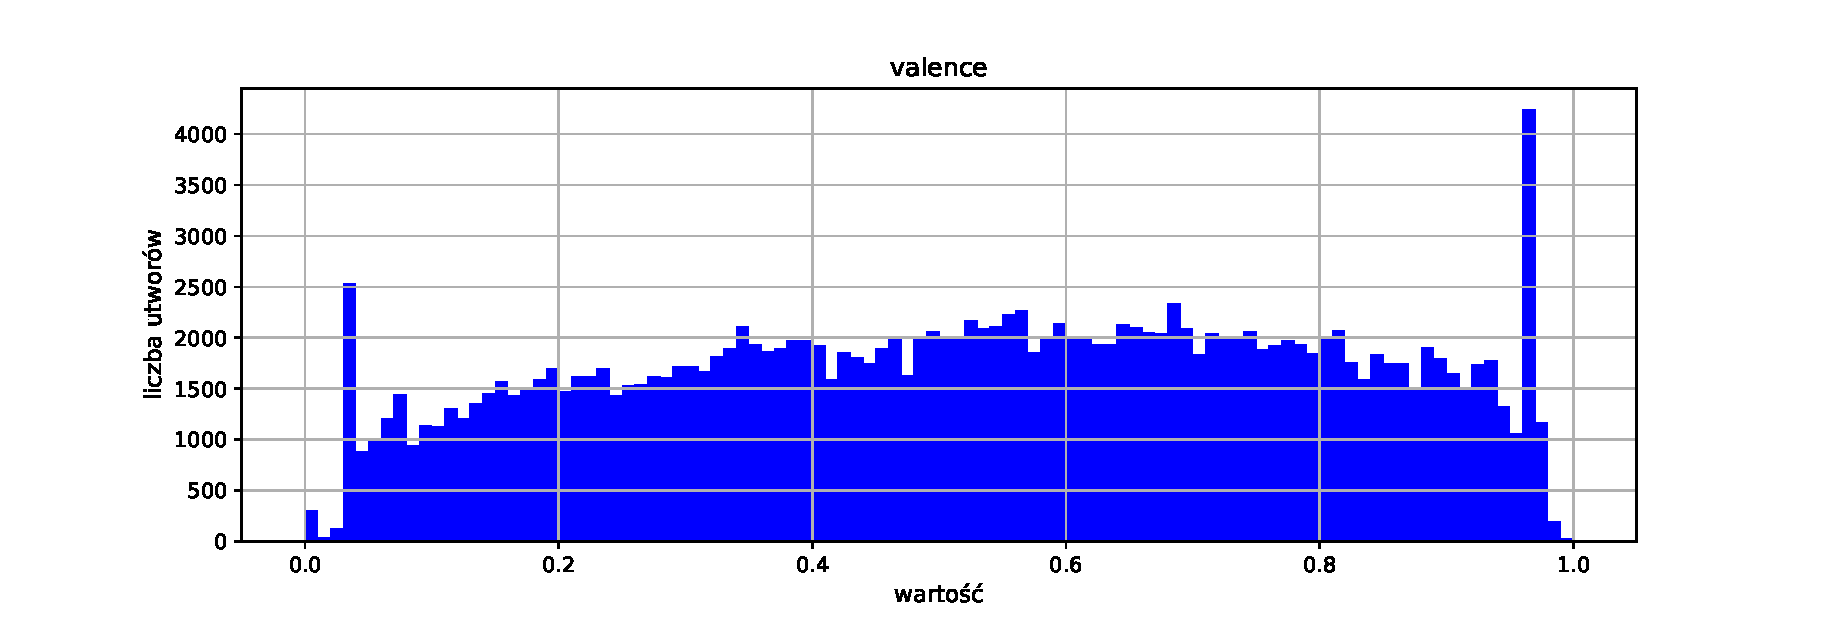
\includegraphics[width=\textwidth]{valence}
        \caption{Histogram dla cechy \textit{valence} (pl. ozdobnik).}
    \end{figure}

    \begin{figure}[H]
        \label{fig:acousticness}
        \centering
        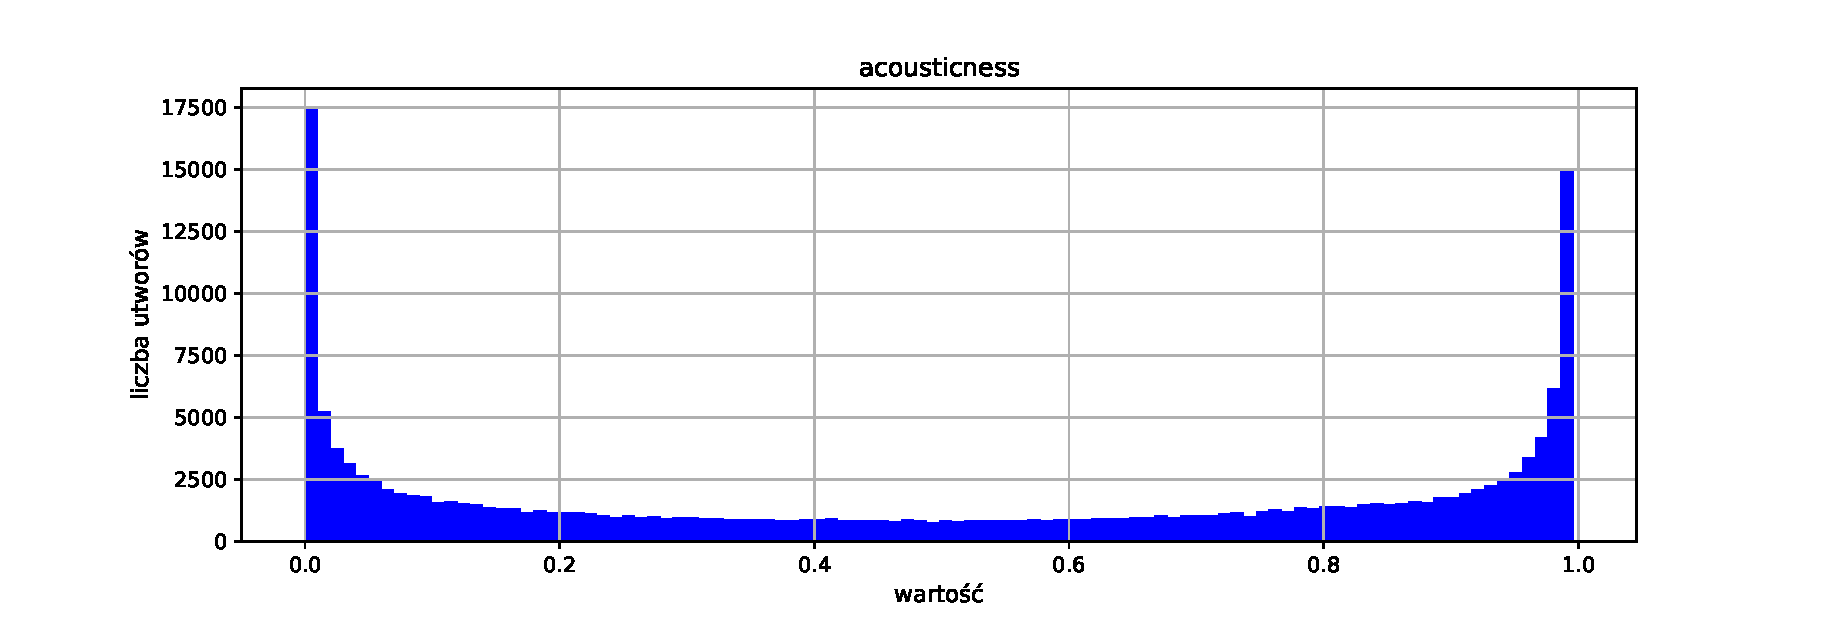
\includegraphics[width=\textwidth]{acousticness}
        \caption{Histogram dla cechy \textit{acousticness} (pl. akustyczność).}
    \end{figure}

    \begin{figure}[H]
        \label{fig:danceability}
        \centering
        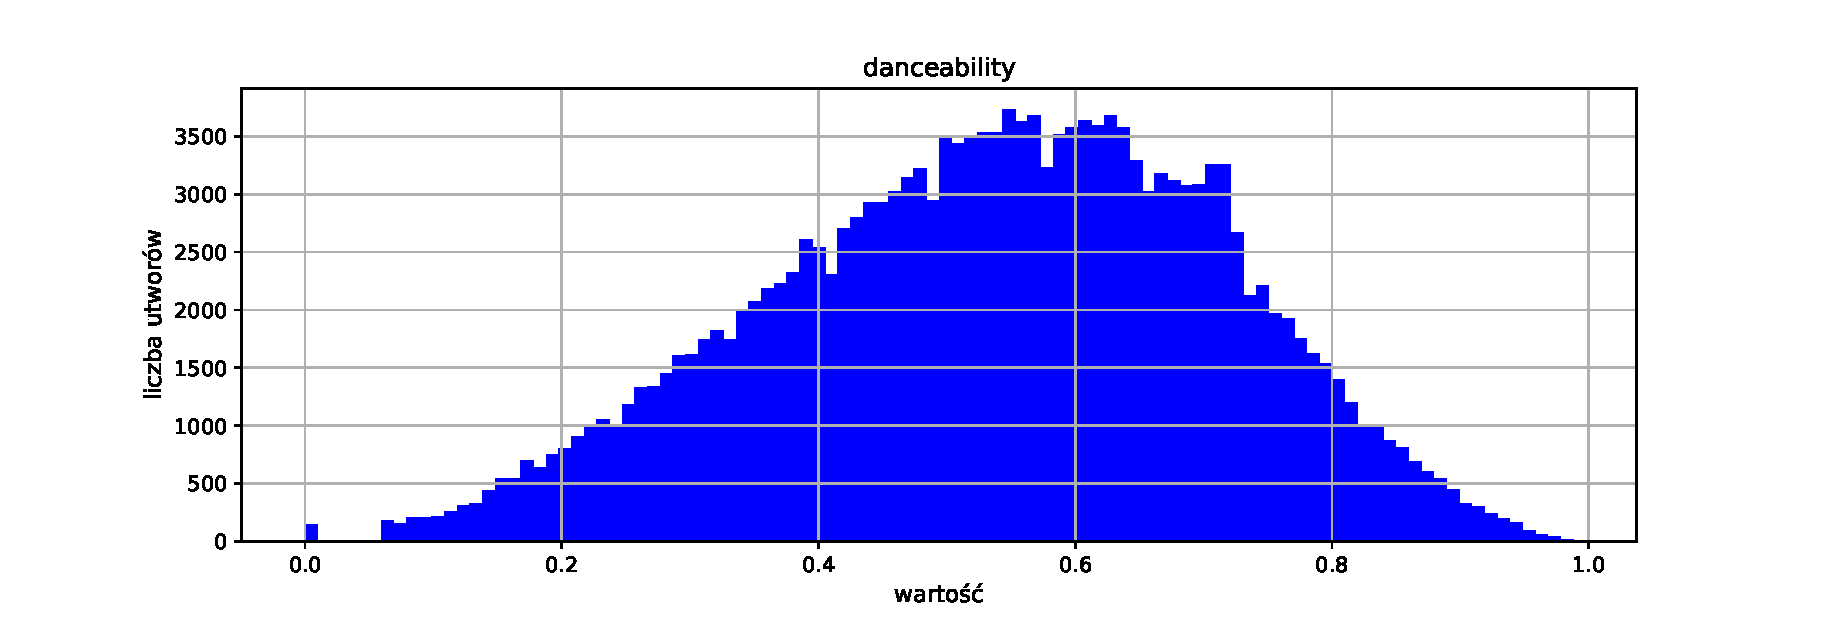
\includegraphics[width=\textwidth]{danceability}
        \caption{Histogram dla cechy \textit{danceability} (pl. taneczność).}
    \end{figure}

    \begin{figure}[H]
        \label{fig:duration_ms}
        \centering
        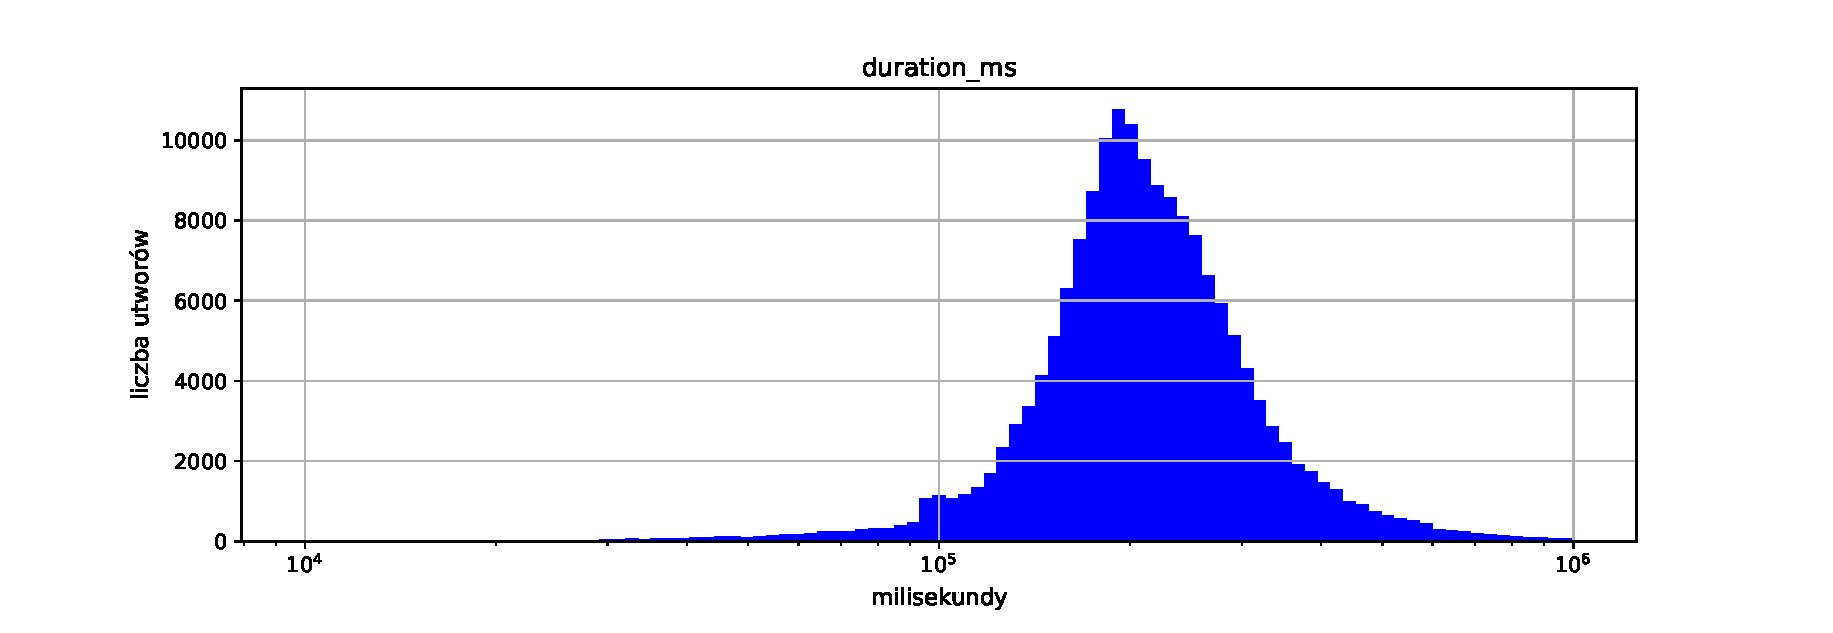
\includegraphics[width=\textwidth]{duration_ms}
        \caption{Histogram dla cechy \textit{duration\_ms} (pl. czas trwania w milisekundach).}
    \end{figure}

    \begin{figure}[H]
        \label{fig:energy}
        \centering
        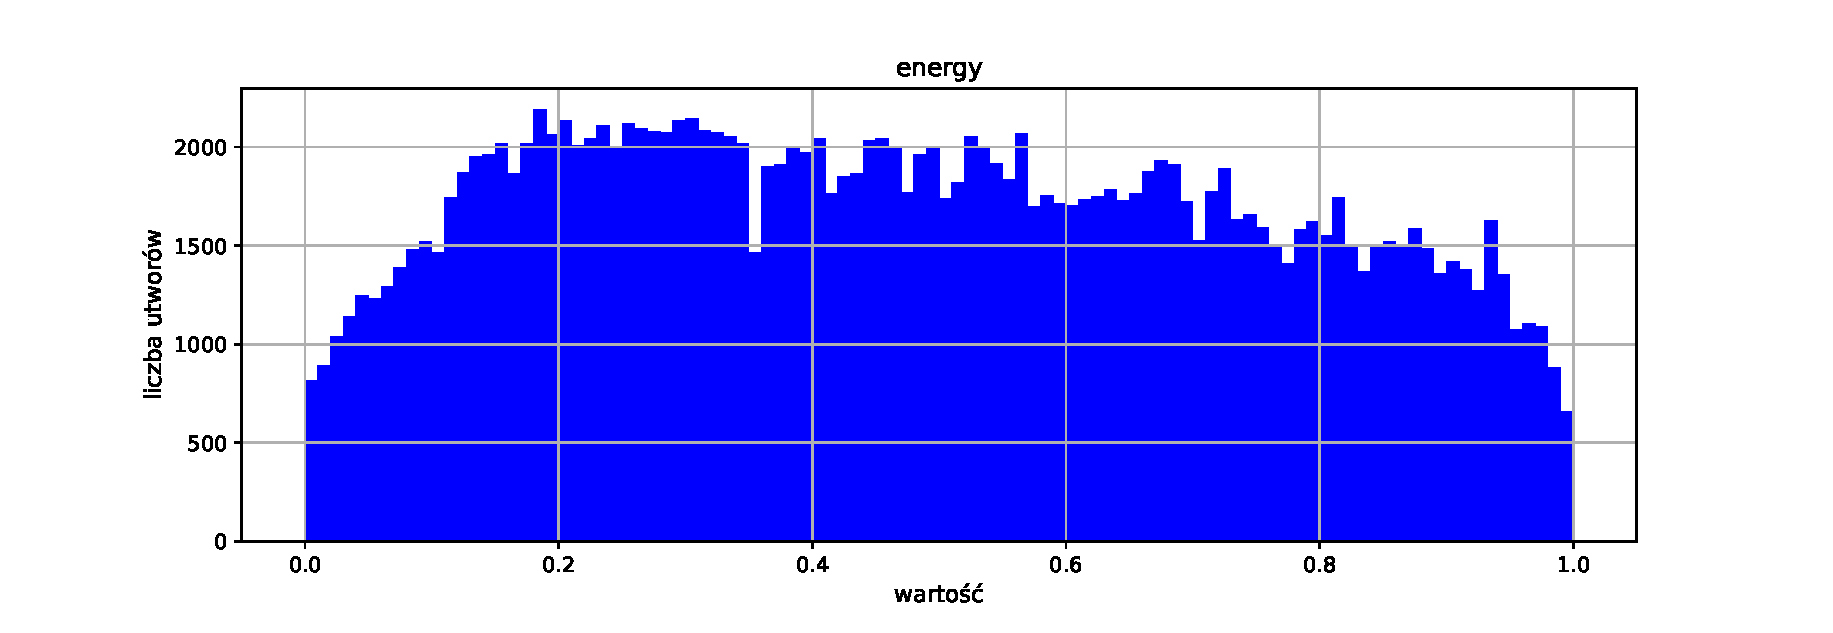
\includegraphics[width=\textwidth]{energy}
        \caption{Histogram dla cechy \textit{energy} (pl. energia/energetyczność).}
    \end{figure}

    \begin{figure}[H]
        \label{fig:instrumentalness}
        \centering
        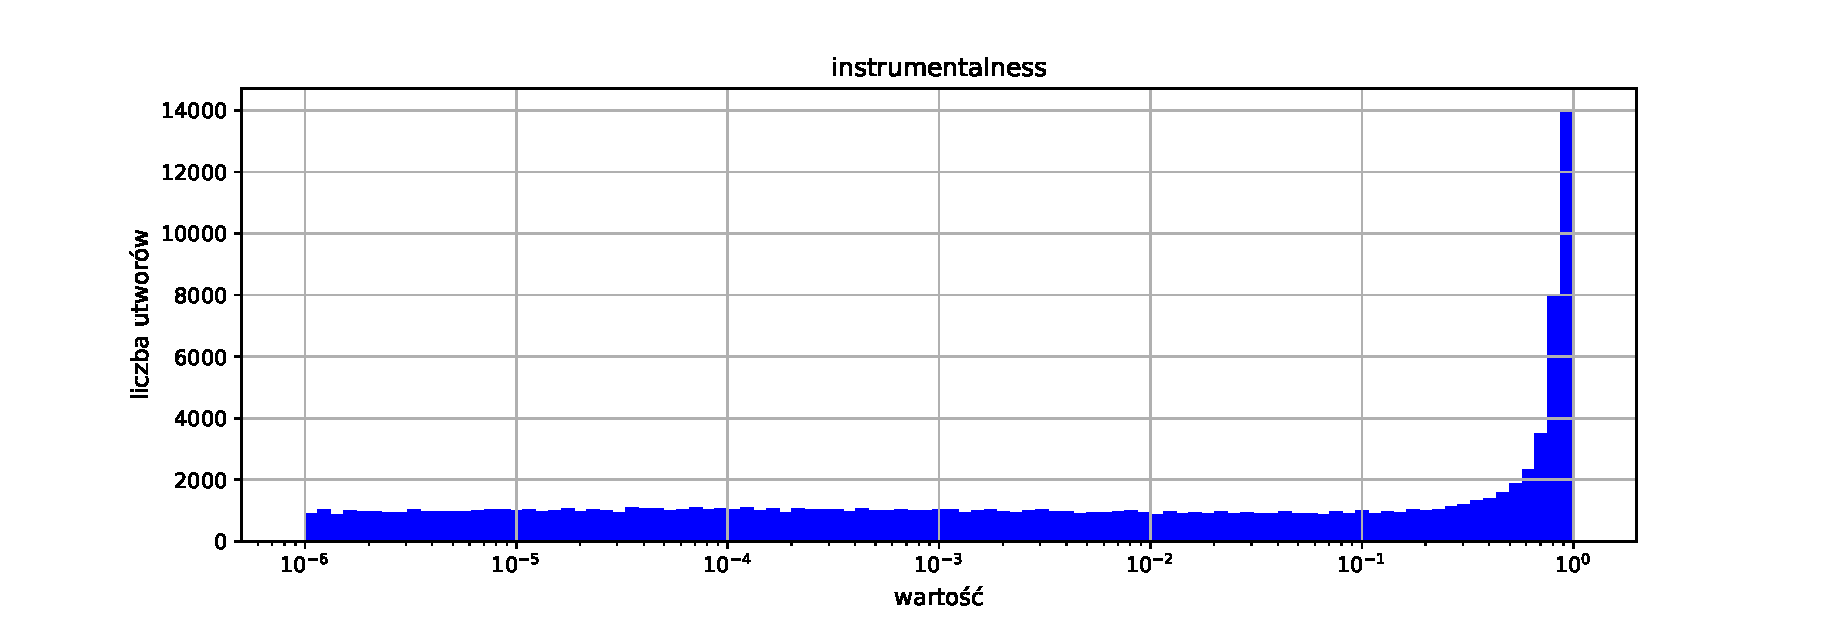
\includegraphics[width=\textwidth]{instrumentalness}
        \caption{Histogram dla cechy \textit{instrumentalness} (pl. instrumentalność).}
    \end{figure}

    \begin{figure}[H]
        \label{fig:liveness}
        \centering
        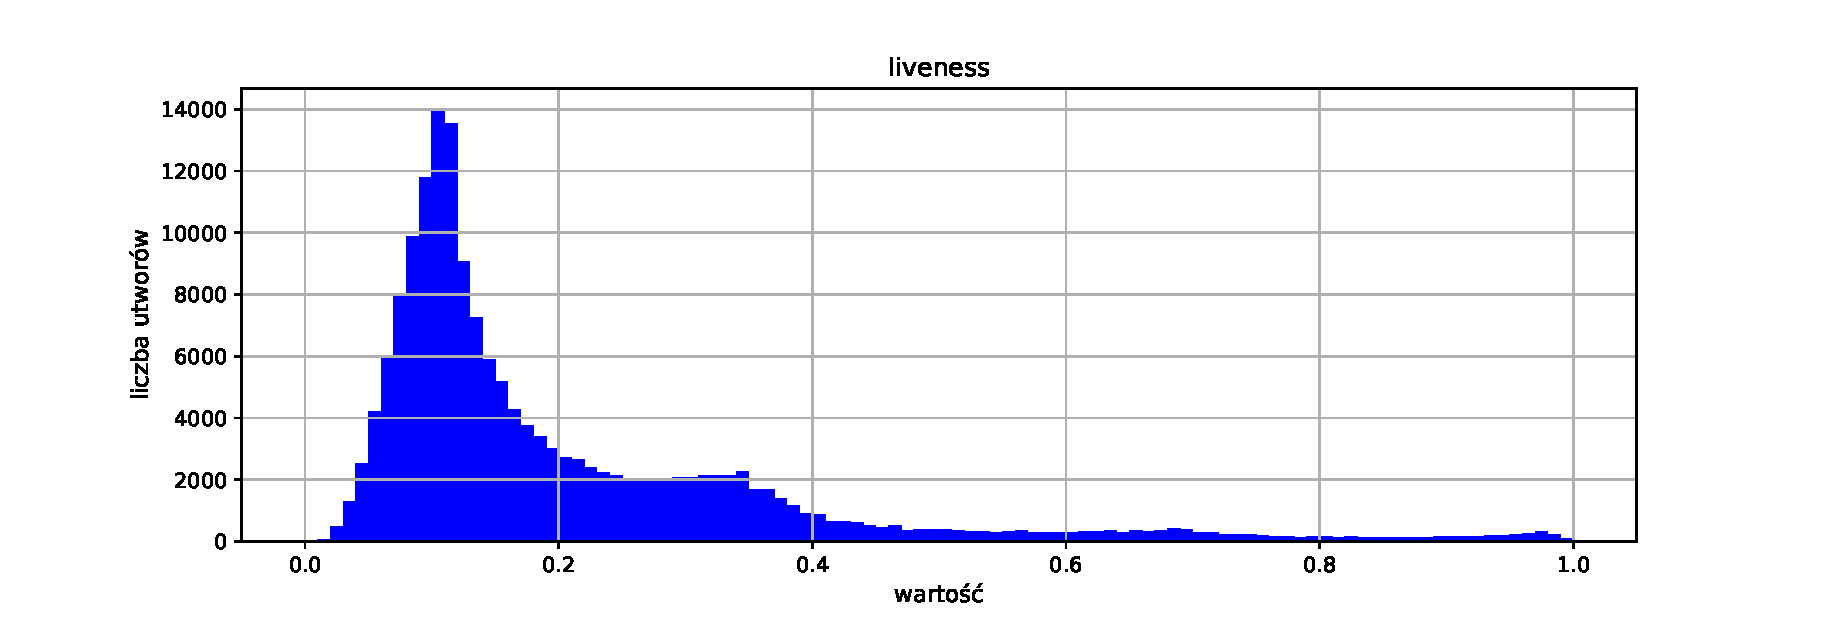
\includegraphics[width=\textwidth]{liveness}
        \caption{Histogram dla cechy \textit{liveness} (pl. żywość/żywiołowość).}
    \end{figure}

    \begin{figure}[H]
        \label{fig:loudness}
        \centering
        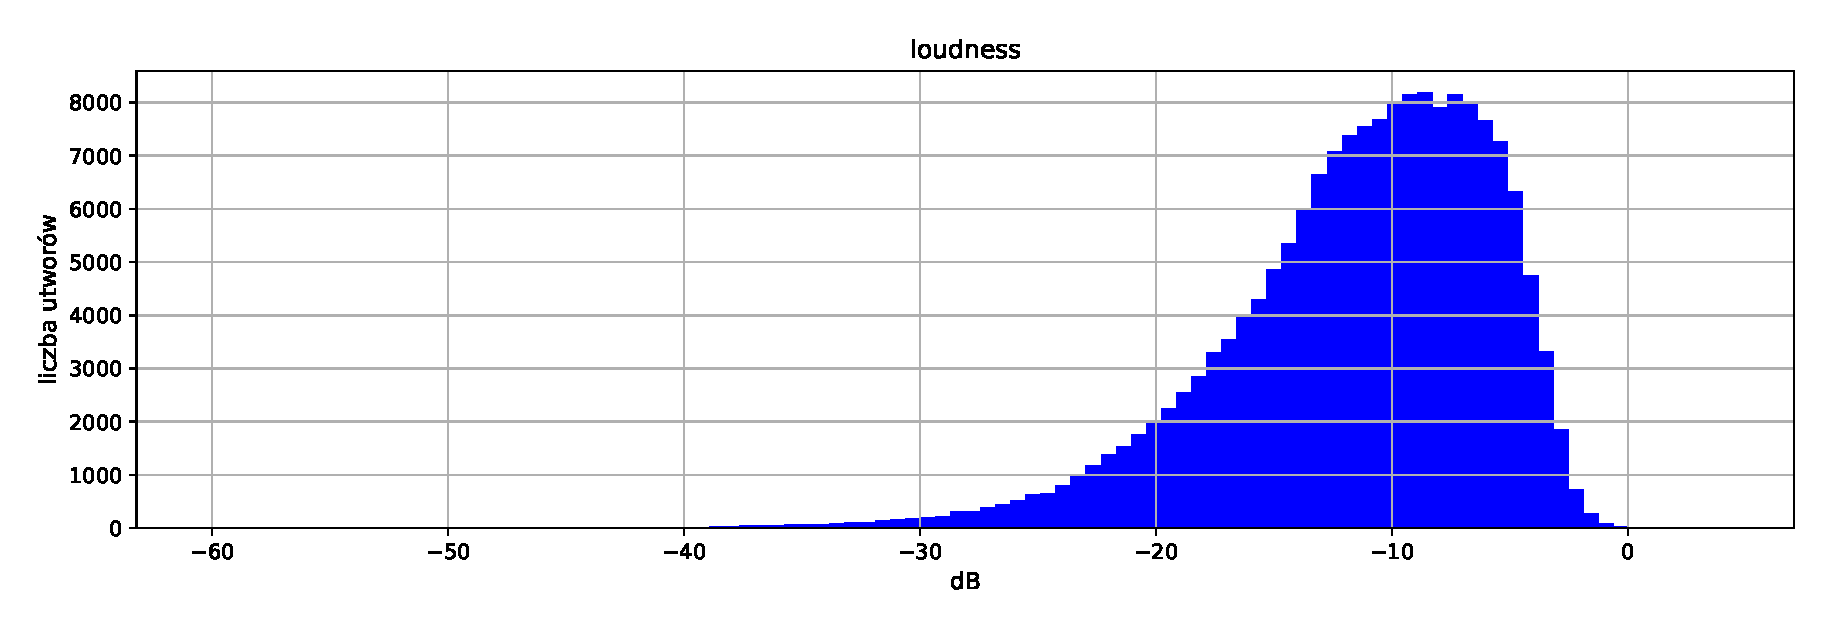
\includegraphics[width=\textwidth]{loudness}
        \caption{Histogram dla cechy \textit{loudness} (pl. głośność).}
    \end{figure}

    \begin{figure}[H]
        \label{fig:year}
        \centering
        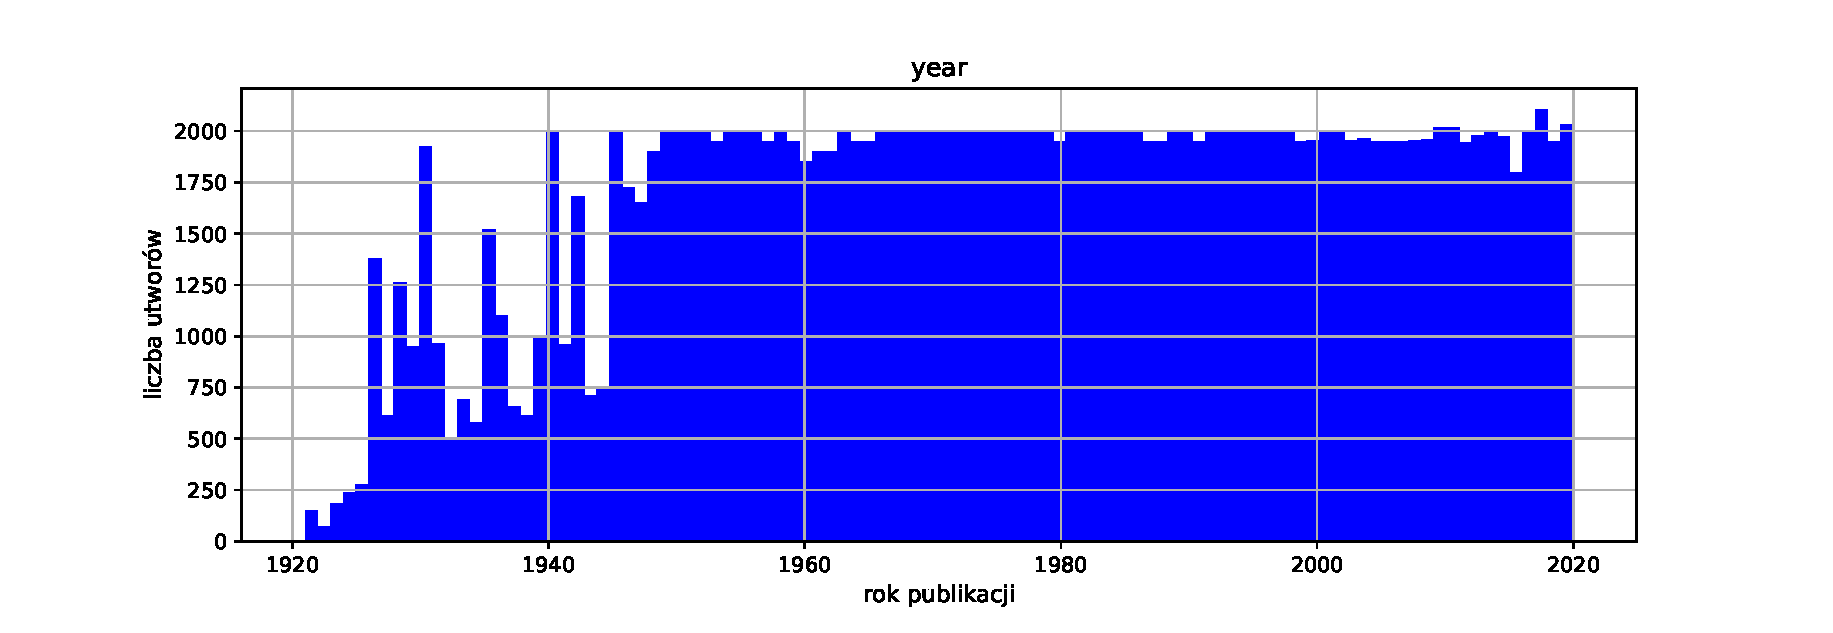
\includegraphics[width=\textwidth]{year}
        \caption{Histogram dla cechy \textit{year} (pl. rok publikacji).}
    \end{figure}

    \begin{figure}[H]
        \label{fig:speechiness}
        \centering
        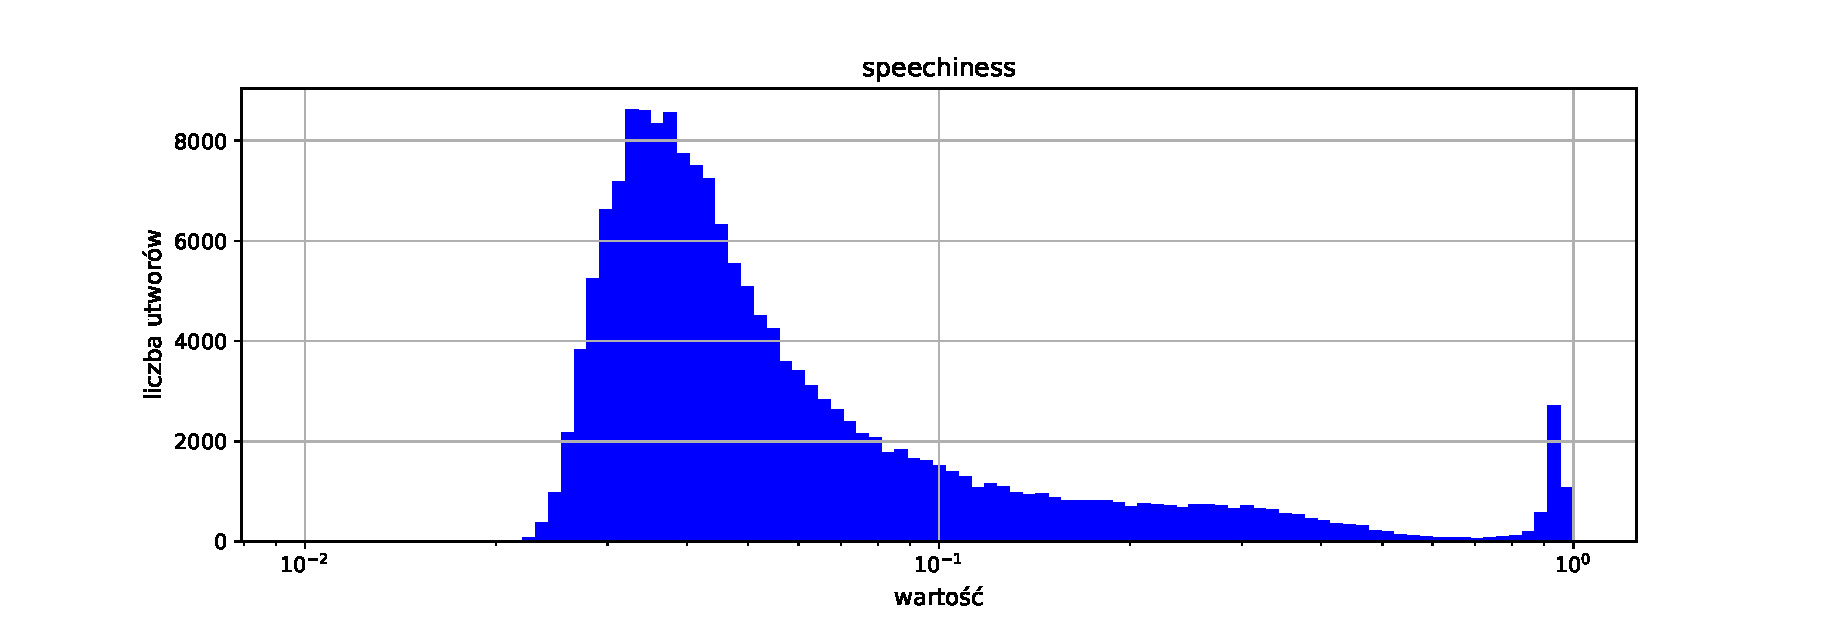
\includegraphics[width=\textwidth]{speechiness}
        \caption{Histogram dla cechy \textit{speechiness} (pl. wypełnienie mową).}
    \end{figure}

    \begin{figure}[H]
        \label{fig:tempo}
        \centering
        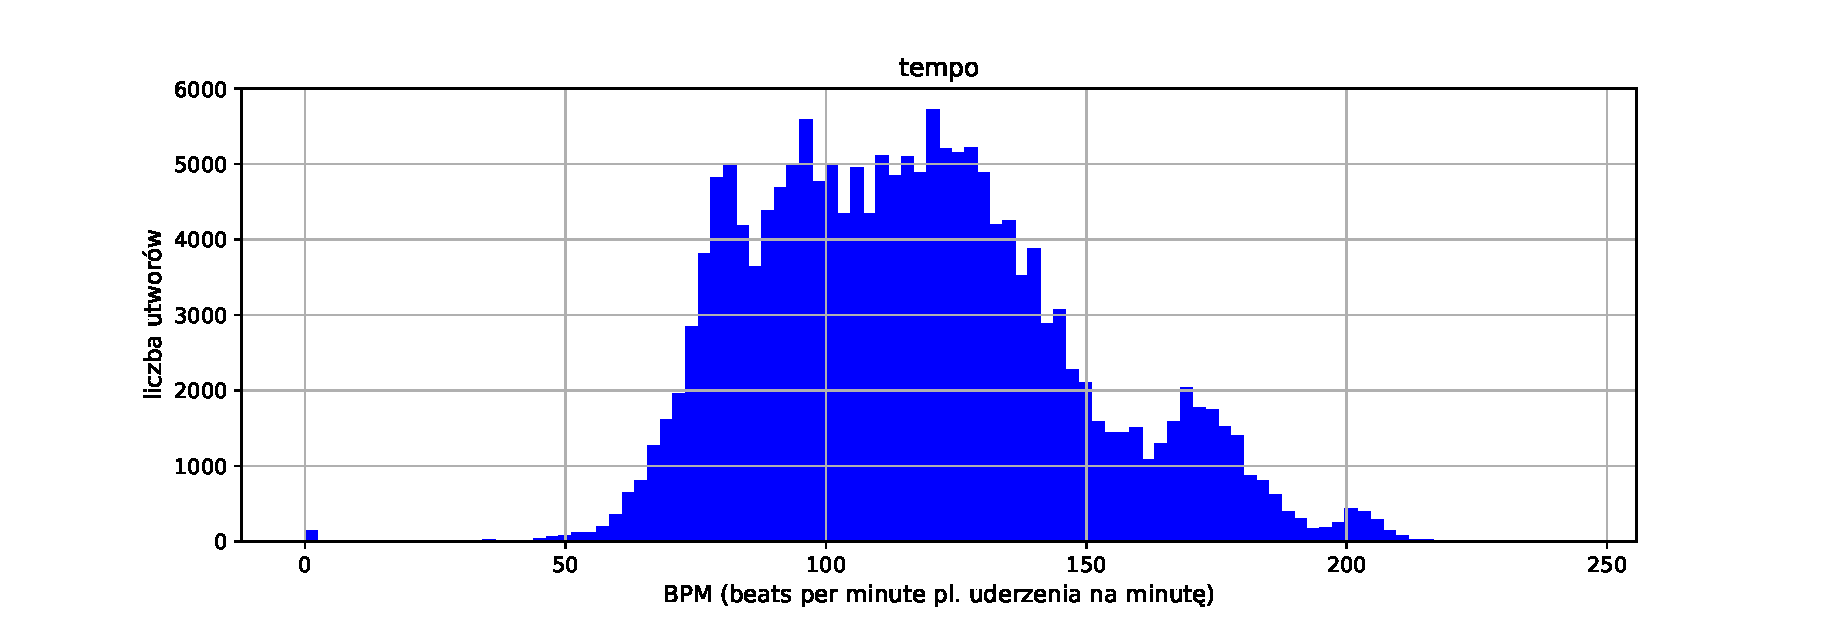
\includegraphics[width=\textwidth]{tempo}
        \caption{Histogram dla cechy \textit{tempo} (pl. tempo).}
    \end{figure}

    \begin{figure}[H]
        \label{fig:mode}
        \centering
        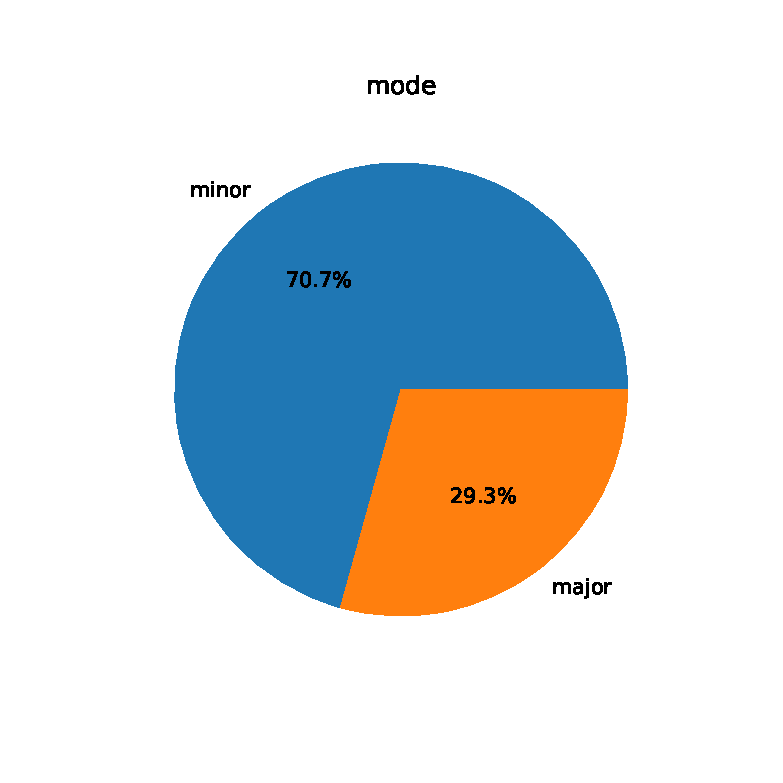
\includegraphics[width=7cm,keepaspectratio]{mode}
        \caption{Wykres kołowy pokazujący procentowy rozkład dominant dla badanych utworów.}
    \end{figure}

    \begin{figure}[H]
        \label{fig:explicit}
        \centering
        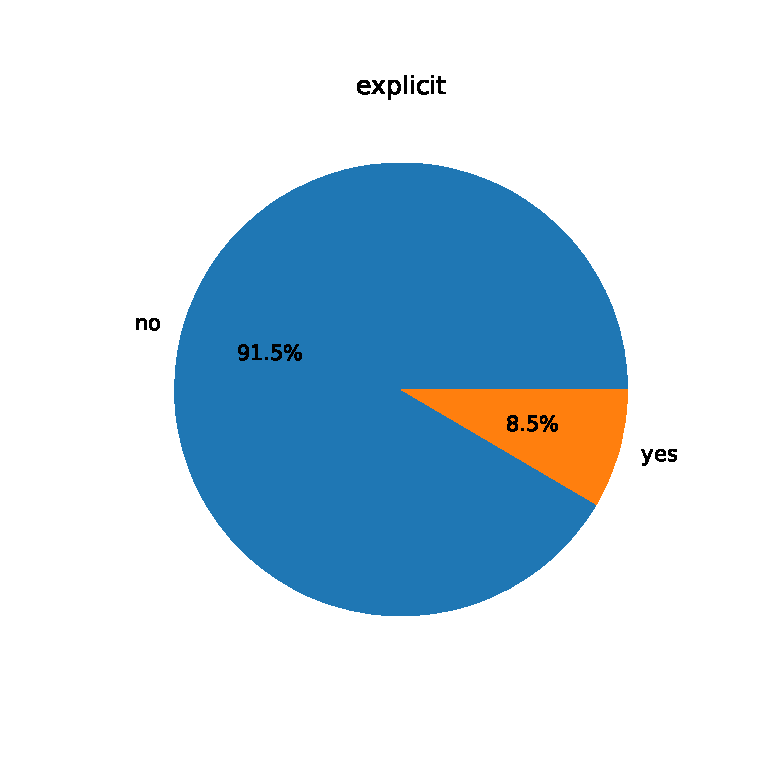
\includegraphics[width=7cm,keepaspectratio]{explicit}
        \caption{Wykres kołowy pokazujący procentowy udział utworów zawierających treści przeznaczone dla odbiorców pełnoletnich.}
    \end{figure}

    \begin{figure}[H]
        \label{fig:key}
        \centering
        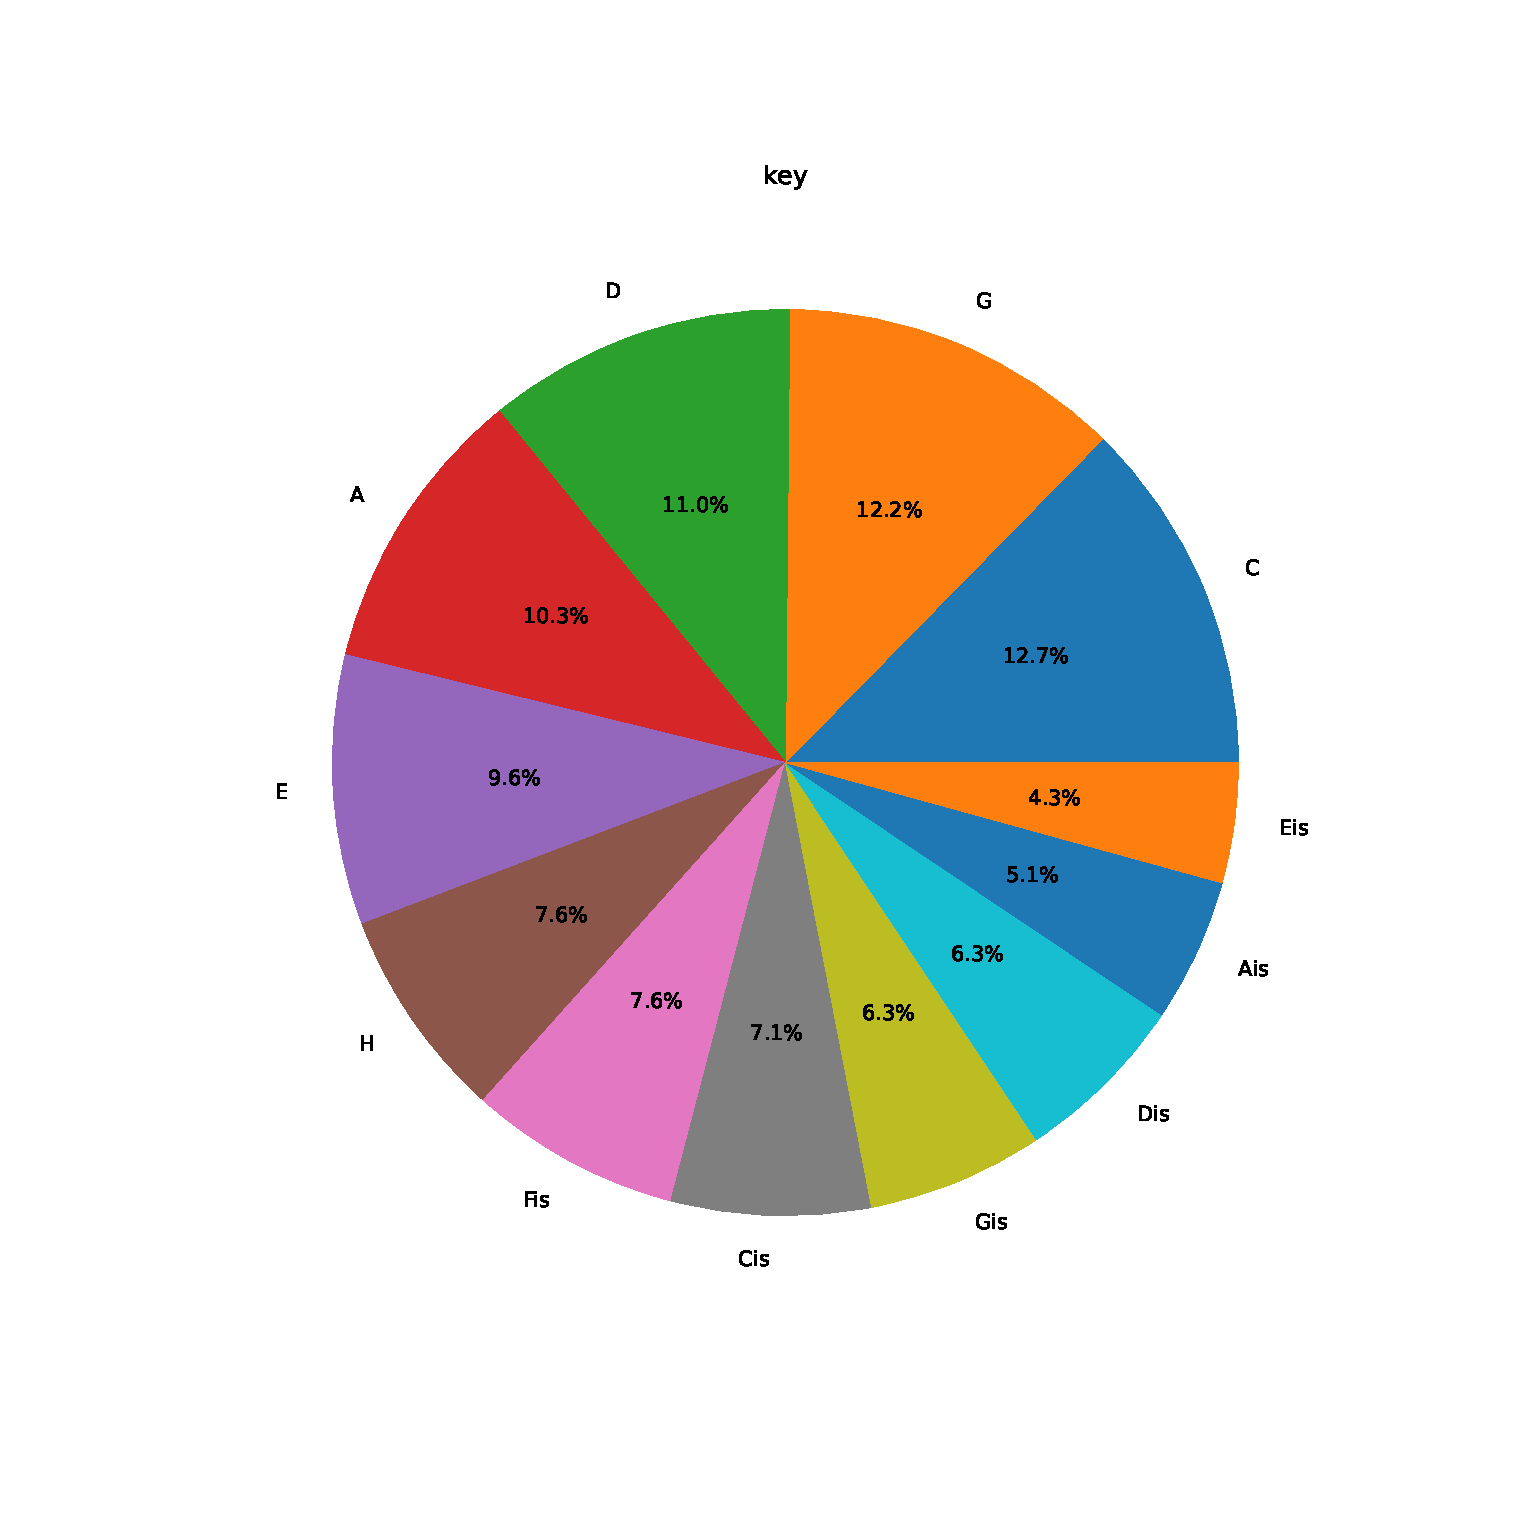
\includegraphics[width=10cm,keepaspectratio]{key}
        \caption{Wykres kołowy pokazujący procentowy rozkład tonacji dla badanych utworów.}
    \end{figure}

    \bigskip

    Do stworzenia modeli wykorzystano następujące parametry: \textit{valence}, \textit{acousticness}, \textit{danceability}, \textit{duration\_ms}, \textit{energy}, \textit{explicit}, \textit{instrumentalness}, \textit{key}, \textit{liveness}, \textit{loudness}, \textit{mode}, \textit{release\_date}, \textit{speechiness} i \textit{tempo} Trzeba tu nadmienić, że na potrzeby dalszych działań wartości parametru \textit{key} zostały zamienione na binarną postać wektorową (ang. \textit{one-hot encoding}), a wartości \textit{release\_date} na milisekundy w standardzie UNIX. Na podstawie wartości wcześniej wymienionych parametrów modele szacowały wartość popularności (ang. \textit{popularity}) utworu.


    \section{Zastosowanie dwustopniowego algorytmu uczenia maszynowego do predykcji popularności utworu}

    \subsection{Wstępna obróbka danych}

    \subsection{Ogólny zarys architektury zastosowanej sieci neuronowej}

    \subsection{Inicjacja wag funkcją HE}

    Podczas badań nad procesem uczenia głębokich sieci neuronowych badacze natrafili na tak zwany `problem zanikających gradientów' (malenie wartości gradientów funkcji kosztu wraz z propagacją wsteczną na coraz niższe warstwy sieci) oraz będący jego przeciwieństwem `problem wybuchających gradientów' (stały wzrost gradientów powodujący rozbieżność algorytmu, problem dotyczący głównie rekurencyjnych sieci neuronowych)\cite{UczenieMaszynowe2018}. Była to przeszkoda na tyle poważna, że na długie lata wstrzymała rozwój prac nad głębokimi sieciami neuronowymi. Dopiero w 2010 roku Xavier Glorot i Yoshua Benglo udało się zdiagnozować przyczynę problemu i zaproponować skuteczne rozwiązanie. Przyczyną okazało się być powszechne wykorzystywanie kombinacji logistycznej i sigmoidalnej funkcji aktywacji oraz inicjacji wag losowymi wartościami o rozkładzie normalnym i średniej równej 0 oraz odchyleniu standardowym równym 1. Badacze doszli do wniosku, że prawidłowy przepływ informacji między warstwami sieci jest możliwy jedynie gdy wariancja dla wyjść warstwy jest równa wariancji wejść tejże, a także gradienty funkcji kosztu muszą mieć taką samą wariancję przed i po przejściu przez daną warstwę w procesie propagacji wstecznej\cite{UnderstandingTheDifficultyOfTrainingDeepFeedforwardNeuralNetworks2010}.

    \bigskip

    Wzory dla inicjacji Xaviera (Glorot), dla logistycznej funkcji aktywacji przedstawiają się następująco:

    \bigskip

    Odchylenie standardowe dla rozkładu normalnego o średniej 0:
    \begin{equation}
        \label{equ:std_dev_xavier}
        \sigma = \sqrt{\frac{2}{n_{input} + n_{output}}}
    \end{equation}

    \smallskip

    Promień dla rozkładu jednorodnego (gdzie wartości mieszczą się w przedziale $\langle$-r,r$\rangle$):
    \begin{equation}
        \label{equ:radius_xavier}
        r = \sqrt{\frac{6}{n_{input} + n_{output}}}
    \end{equation}

    \bigskip

    \begin{tabular}{p{0.08\textwidth}p{0.92\textwidth}}
        Gdzie: \\
        n\textsubscript{input}  & liczba połączeń wejściowych w warstwie \\
        n\textsubscript{output} & liczba połączeń wyjściowych w warstwie \\
    \end{tabular}

    \bigskip

    Zaproponowana przez Glorot i Benglo metoda inicjacji wag sprawdzała się świetnie w połączeniu z logistyczną funkcją aktywacji. W przypadku zastosowania jej w połączeniu z funkcją aktywacji ReLU (a także jej odmianami takimi jak ELU) wyniki były niezadowalające. Kolejnego przełomu udało się dokonać w 2015 roku Kaiming He wraz zespołem współpracowników z Microsoft Research w wyniku prac nad klasyfikatorem dla zbioru ImageNet\cite{DelvingDeepIntoRectifiers2015}. Inicjacja He w odróżnieniu od inicjacji Xaviera (Glorot) uwzględnia jedynie obciążalność wejściową warstwy (a nie jak u poprzednika średnią obciążalności wejściowej i wyjściowej)\cite{UczenieMaszynowe2018}.

    \bigskip

    Wzór na odchylenie standardowe w inicjacji He dla rozkładu normalnego o średniej 0:

    \begin{equation}
        \label{equ:std_dev_he}
        \sigma = \sqrt{\frac{2}{n_{input}}}
    \end{equation}

    \bigskip

    \begin{tabular}{p{0.08\textwidth}p{0.92\textwidth}}
        Gdzie: \\
        n\textsubscript{input} & liczba połączeń wejściowych w warstwie \\
    \end{tabular}

    \subsection{Funkcja aktywacji ELU}

    Początkowo uważano, że najlepsze jako funkcje aktywacji będą funkcje sigmoidalne. Przekonanie to brało się stąd, że podobnymi funkcjami można opisać przetwarzanie sygnału przez neurony biologiczne. To intuicyjne skojarzenie okazało się jednak mylne. Po pewnym czasie odkryto, że o wiele lepiej do tego celu nadaje się funkcja ReLU(ang. \textit{Rectified Linear Unit} pl. prosta liniowa funkcja aktywacji)\cite{UczenieMaszynowe2018}. Głównymi zaletami funkcji ReLU są:
    \begin{itemize}
        \item nie uleganie nasyceniu dla wartości dodatnich
        \item ma bardzo niski koszt obliczeniowy
    \end{itemize}

    \bigskip

    Wzór dla funkcji aktywacji ReLU:
    \begin{equation}
        ReLU(x) =
        \begin{cases}
            0 & \quad \text{jeśli } x < 0 \\
            x & \quad \text{jeśli } x \geq 0
        \end{cases}
    \end{equation}

    \begin{figure}[H]
        \label{fig:relu}
        \centering
        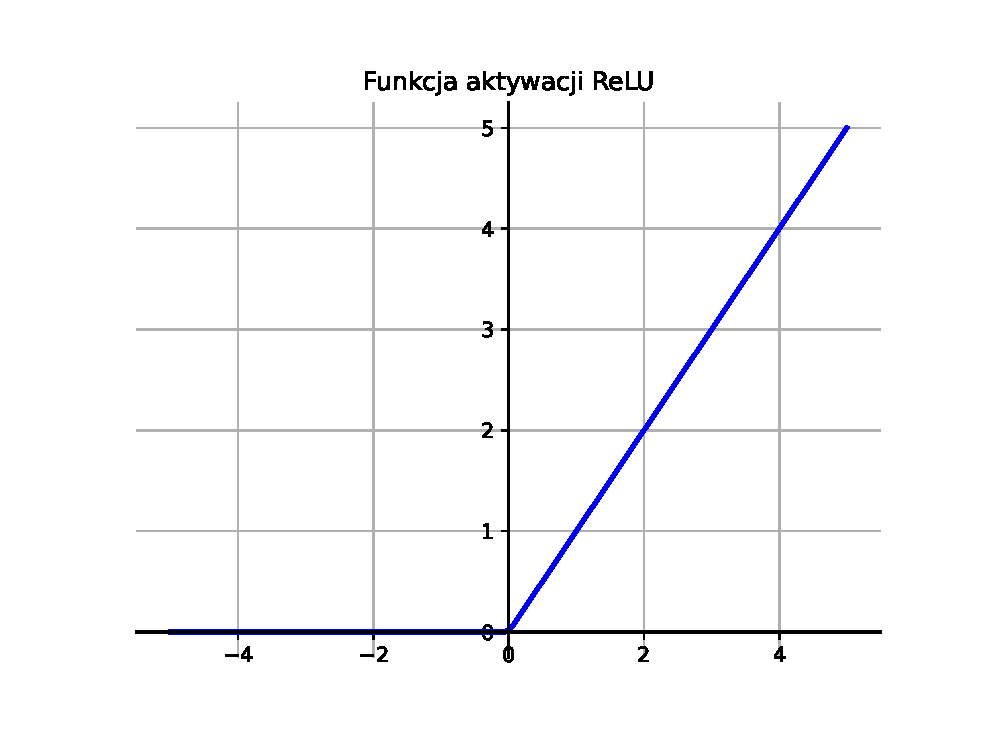
\includegraphics[width=\textwidth]{relu}
        \caption{Wykres funkcji ReLU.}
    \end{figure}

    \bigskip

    Funkcja ReLU ma jednak ogromną wadę, potocznie nazywaną `śmiercią ReLU' - polega to na tym, że w procesie uczenia niektóre neurony trwale `giną', to znaczy że zaczynają przesyłać wyłącznie sygnał 0 i nie ma możliwości, żeby `zmartwychwstały'\cite{UczenieMaszynowe2018}. Z tego też powodu w praktyce stosowane są obecnie modyfikacje funkcji ReLU, z pośród który najpopularniejsze to:
    \begin{itemize}
        \item `przeciekająca' funkcja ReLU
        \item losowa `przeciekająca' funkcja ReLU
        \item parametryczna `przeciekająca' funkcja ReLU
        \item ELU (ang. \textit{exponential linear unit} pl. jednostka wykładniczo liniowa)
    \end{itemize}

    \bigskip

    W 2015 roku Djork-Arné Clevert wraz z zespołem odkrył nową funkcję aktywacji - ELU\cite{FastAndAccurateDeepNetworkLearningByELU2016}. Po przeprowadzonych eksperymentach okazało się, że góruje ona zarówno nad tradycyjną funkcją ReLU, jak i jej modyfikacjami. Umożliwiała skrócenie procesu uczenia, a także przyczyniła się wydatnie do poprawy wyników dla zbioru testowego\cite{UczenieMaszynowe2018}. Główne zalety ELU w zestawieniu z ReLU to:
    \begin{itemize}
        \item rozwiązanie `problemu zanikających gradientów' dzięki przyjmowaniu ujemnych wartości dla x < 0
        \item rozwiązanie problemu `umierających neuronów' dzięki niezerowemu gradientowi dla x < 0
        \item przyspieszenie procesu uczenia metodą gradientu prostego dzięki gładkości funkcji na cały przebiegu
    \end{itemize}

    \smallskip

    Wadą jest natomiast niewątpliwie większy koszt obliczeniowy w porównaniu z ReLU spowodowany obecnością składowej wykładniczej.

    \bigskip

    Wzór dla funkcji aktywacji ELU:
    \begin{equation}
        ELU_{\alpha}(x) =
        \begin{cases}
            \alpha(\exp(x)-1) & \quad \text{jeśli } x < 0 \\
            x & \quad \text{jeśli } x \geq 0
        \end{cases}
    \end{equation}

    \bigskip

    \begin{tabular}{p{0.08\textwidth}p{0.92\textwidth}}
        Gdzie: \\
        $\alpha$ & hiperparametr definiujący wartość do jakiej ma się zbliżać funkcja dla ujemnych wartości x \\
    \end{tabular}

    \begin{figure}[H]
        \label{fig:elu}
        \centering
        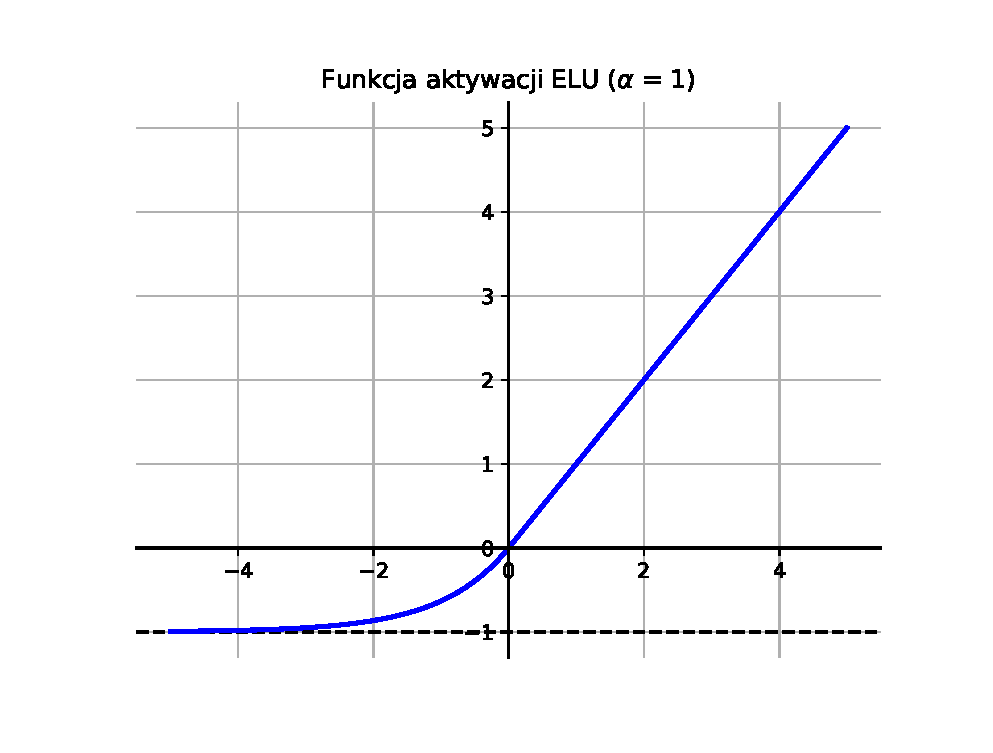
\includegraphics[width=\textwidth]{elu}
        \caption{Wykres funkcji ELU dla $\alpha$=1.}
    \end{figure}

    \subsection{Normalizacja wsadowa (ang. \textit{Batch Normalization})}

    Zastosowanie kombinacji inicjacji He w połączeniu z funkcją aktywacji ELU nie rozwiązało całkowicie problemu zanikających i eksplodujących gradientów. Problem nadal występował na dalszych etapach procesu uczenia. Dopiero zaproponowane w 2015 roku przez Sergeya Ioffe i Christiana Szegedy rozwiązanie - normalizacja wsadowa (ang. \textit{Batch Normalization}), w połączeniu z wcześniej wymienionymi pozwoliło ostatecznie pokonać trudność\cite{BatchNormalization2015}.

    \bigskip

    Operację normalizacji wsadowej wykonuje się na każdej warstwie bezpośrednio przed funkcją aktywacji. Najpierw wyśrodkowuje się i normalizuje się dane wyjściowe. Następnie przeskalowuje się i przesuwa się wyniki za pomocą dwóch parametrów wyliczanych dla każdej warstwy ($\gamma$ - parametr skalowania, $\beta$ - parametr przesunięcia)\cite{UczenieMaszynowe2018}.

    \bigskip

    Algorytm normalizacji wsadowej:

    \bigskip

    Wyliczenie średniej dla minigrupy: \\
    \begin{equation}
        \mu_{B} = \frac{1}{m_{B}} \displaystyle\sum_{i=1}^{m_{B}} x^{(i)}
    \end{equation}

    \smallskip

    Wyliczenie odchylenia standardowego dla minigrupy: \\
    \begin{equation}
        \sigma_{B}^{2} = \frac{1}{m_{B}} \displaystyle\sum_{i=1}^{m_{B}} (x^{(i)} - \mu_{B})^{2}
    \end{equation}

    \smallskip

    Wyśrodkowanie i znormalizowanie danych wejściowych: \\
    \begin{equation}
        \widehat{x}^{(i)} = \frac{x^{(i)} - \mu_{B}}{\sqrt{\sigma_{B}^{2} + \epsilon}}
    \end{equation}

    \smallskip

    Przeskalowanie i przesunięcie wyniku: \\
    \begin{equation}
        z^{(i)} = \gamma\widehat{x}^{(i)} + \beta
    \end{equation}

    \bigskip

    \begin{tabular}{p{0.08\textwidth}p{0.92\textwidth}}
        Gdzie: \\
        $\mu_{B}$           & średnia empiryczna wyliczona dla całej minigrupy B                                                                                                                \\
        $\sigma_{B}$        & empiryczne odchylenie standardowe wyliczone dla całej minigrupy B                                                                                                 \\
        $m_{B}$             & liczba przykładów w minigrupie                                                                                                                                    \\
        $\widehat{x}^{(i)}$ & wyśrodkowane i znormalizowane dane wejściowe                                                                                                                      \\
        $\gamma$            & parametr skalowania w danej warstwie                                                                                                                              \\
        $\beta$             & parametr przesunięcia w danej warstwie                                                                                                                            \\
        $\epsilon$          & niewielka liczba służąca do uniknięcia operacji dzielenia przez 0 (zazwyczaj ma wartość $10^{-5}$; jest to tzw, człon wygładzający (ang. \textit{smoothing term}) \\
        $z^{(i)}$           & wynik operacji normalizacji wsadowej: przeskalowana i przesunięta wersja danych wejściowych                                                                       \\
    \end{tabular}

    \bigskip

    Główne zalety normalizacji wsadowej to\cite{UczenieMaszynowe2018}:
    \begin{itemize}
        \item ograniczenie `problemu zanikających gradientów' w stopniu pozwalającym na używanie nasycających funkcji aktywacji takich jak tangens hiperboliczny
        \item zmniejszenie wrażliwości sieci na inicjację wag
        \item umożliwienie wykorzystywania większej wartości współczynnika uczenia, a co za tym idzie znaczne przyspieszenie całego procesu uczenia
        \item poprawa wyników dla zagadnień klasyfikacji i regresji
        \item częściowe spełnianie roli regularyzatora
    \end{itemize}

    \bigskip

    Największe wady to\cite{UczenieMaszynowe2018}:
    \begin{itemize}
        \item zwiększenie skomplikowania modelu
        \item spowolnienie działania modelu ze względu na konieczność przeprowadzenia dodatkowych obliczeń dla każdej warstwy (spowalnia to w szczególności początek procesu uczenia, gdyż algorytm gradientu prostego wyszukuje optymalne skale i przesunięcia dla każdej warstwy, następnie proces przyspiesza)
    \end{itemize}

    \subsection{Regularyzacja przez Porzucanie (ang. \textit{Dropout})}

    Pierwotny pomysł zastosowania techniki `porzucania' jako sposobu na regularyzację głębokiej sieci neuronowej powstał w 2012 roku. Jego autorem był pracujący na Uniwersytecie Toronto G.E. Hinton (wraz ze współpracownikami). Wyniki swoich badań zaprezentował w artykule ``Improving neural networks by preventing co-adaptation of feature detectors''\cite{ImprovingNeuralNetworks2012}. Jego dzieło rozwinął działający na tej samej uczelni Nitish Srivastava (ze swoim zespołem), a rezultaty opublikował w 2014 roku w artykule ``Dropout: A Simple Way to Prevent Neural Networks from Overfitting''\cite{Dropout2014}. Osiągane rezultaty były imponujące - zwiększenie dokładności klasyfikatorów o 1-2\% co przekładało się na nawet kilkudziesięciu procentowe zmniejszenie współczynnika błędu.

    \bigskip

    Algorytm jest bardzo prosty. Podczas każdego przebiegu procesu uczenia dowolny neuron, za wyjątkiem neuronów warstwy wyjściowej, może zostać `porzucony', to znaczy całkowicie pominięty w procesie uczenia, z ustalonym z góry prawdopodobieństwem \textit{p}. Następnie już po zakończeniu treningu konieczne jest przemożenie każdej wagi połączenia wejściowego przez tak zwane `prawdopodobieństwo utrzymania' (ang. \textit{keep probability}) równe 1 - \textit{p}. Alternatywą jest podzielenie wartości wejścia każdego neuronu przez `prawdopodobieństwo utrzymania' w trakcie nauki\cite{UczenieMaszynowe2018}.

    \bigskip

    W praktyce dla każdej `epoki' mamy do czynienia z unikalną siecią. Istnieje $2^{N}$ możliwych kombinacji gdzie N oznacza całkowitą liczbę neuronów, które mogą zostać porzucone. Te sztucznie pomniejszone sieci są wobec siebie całkowicie niezależne. Finalna sieć jest pewnym rodzajem uśrednienia\cite{UczenieMaszynowe2018}.

    \bigskip

    Podsumowując, główne korzyści płynące z zastosowania techniki `porzucania' to\cite{UczenieMaszynowe2018}:
    \begin{itemize}
        \item uczone neurony nie mogą uzależniać się od swoich sąsiadów; same muszą wnosić jak najwięcej `wartości dodanej' przy przetwarzaniu sygnału; muszą skupiać się na poszczególnych wejściach, a nie traktować ich kombinacji całościowo
        \item wynikające z powyższego zmniejszenie wrażliwości na drobne zmiany na wejściach
        \item patrząc całościowo uzyskany w wyniku `porzucania' model jest lepszą generalizacją
    \end{itemize}

    Główną wadą jest spowolnienie procesu konwergencji modelu\cite{UczenieMaszynowe2018}.

    Bardzo ważny jest prawidłowy dobór `współczynnika porzucania' tak, żeby uniknąć zarówno niedotrenowania (zbyt duża wartość) jak i przetrenowania (zbyt mała wartość). Cenną wskazówką jest zastosowanie większej wartości współczynnika dla rozbudowanych warstw, a mniejszej dla niewielkich.

    \bigskip

    \begin{figure}[H]
        \label{fig:dropout}
        \centering
        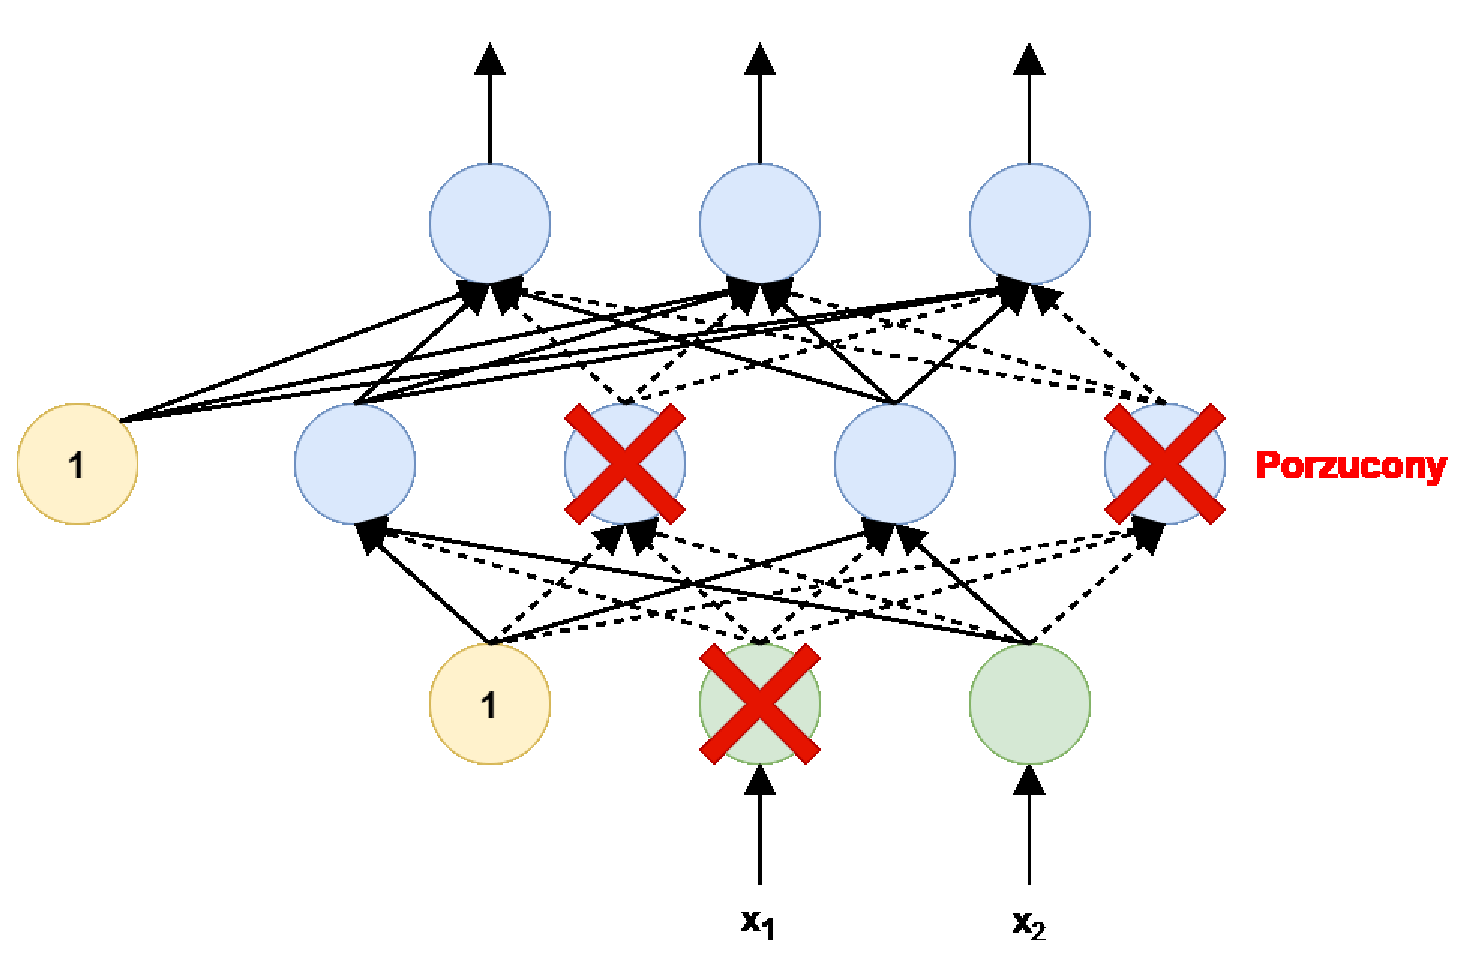
\includegraphics[width=\textwidth]{dropout}
        \caption{Regularyzacja przez `porzucanie'\cite{UczenieMaszynowe2018}.}
    \end{figure}

    \subsection{Optymalizator Adam}

    \subsection{Wybór hiperparametrów procesu uczenia sieci neuronowej}

    \subsection{Wybór rodziców z wykorzystaniem \textit{Fitness Proportionate Selection} (pl. selekcja proporcjonalna) (wariant \textit{Roulette Wheel Selection} (pl. selekcja kołowa))}

    \subsection{Krzyżówka \textit{One Point Crossover} (pl. krzyżówka z jednym punktem przecięcia)}

    \subsection{Mutacja \textit{Bit Flip Mutation} (pl. mutacja przez przerzucenie bitu)}


    \section{Rezultaty eksperymentów}


    \section{Wnioski}


    \printbibliography

\end{document}